\chapter{The Finite Square Well}

\section{Bound States}

What happens if the walls of our ``box'' weren't quite so high?  Let's find out -- suppose we have a particle in a \emph{finite} square well, defined by the potential energy
\begin{equation}
V(x) = \begin{cases}
V_0, \quad x<-a \\
0, \quad -a<x<a \\
V_0, \quad x>a,
\end{cases}
\end{equation}
where $V_0$ is a positive constant -- the depth of the well as shown in Figure \ref{fig_finite_sqr_well_potential}.  Notice one other difference from the infinite version as well: the well has been centered at $x=0$ so the width of the well is actually $2a$; we'll see why in a little bit. 

\begin{figure}
\centering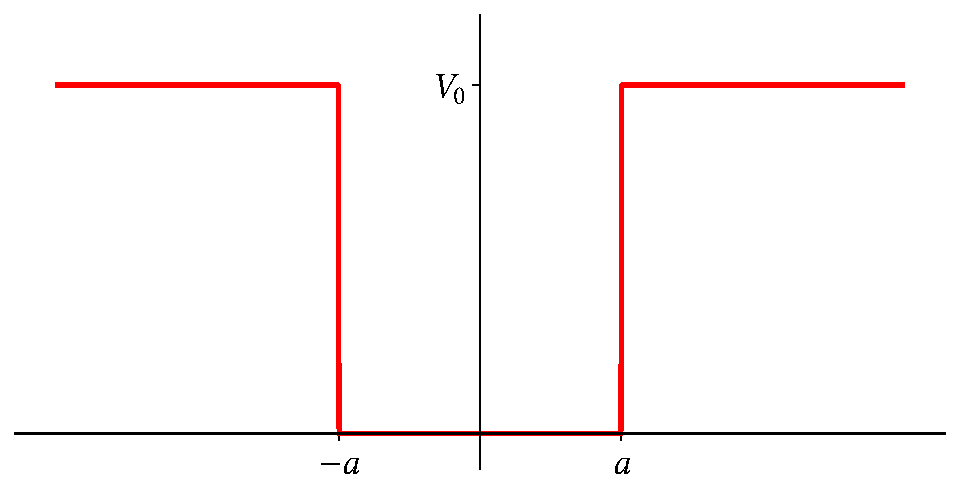
\includegraphics[width=0.7\linewidth]{Figures/Chapter 10/fig_finite_sqr_well_potential.pdf}
\caption{The potential energy of the finite square well.}
\label{fig_finite_sqr_well_potential}
\end{figure}

Actually, probably the biggest difference between the infinite square well and the finite well is what kind of states are allowed.  Classically, for the infinite square well, the particle in the box was always contained and could never escape, regardless of the energy of the particle.  In the finite well, though, if $E>V_0$ the particle would not be trapped in the box and would instead escape to infinity.  As we discussed back in Chapter 8, this case would be an \emph{unbound state}, and unbound states have some additional complications in quantum mechanics -- we'll save those for a later chapter.  In the meantime, we'll only look for bound energy eigenstates, where
\[
E < V_0 \quad \text{(bound states)},
\]
but keep in mind that we'll be missing some of the eigenstates.  One consequence of this is that the energy eigenstates we find here won't be \emph{complete}.

Luckily, finding the bound states is pretty easy.  For $x < -a$, to the left of the well, the energy eigenvalue equation reads
\[
-\frac{\hbar^2}{2m} \frac{d^2 \phi}{dx^2} + V_0 \phi = E\phi,
\]
or, cleaning it up a bit,
\begin{equation}
\frac{d^2\phi}{dx^2} = q^2 \phi,
\end{equation}
where
\begin{equation}
q = \frac{\sqrt{2m(V_0 - E)}}{\hbar}.
\end{equation}
Notice that $q$ is always \emph{real} since we're requiring that $E<V_0$.  This should be a recognizable differential equation; the general solution looks like
\begin{equation}
\phi(x) = A e^{qx} + B e^{-qx} \quad \text{($x<-a$)}.
\end{equation}
Similarly, for $x>a$, the potential energy is again $V = V_0$ so our solution is the same, although we'll have to use different constants:
\begin{equation}
\phi(x) = F e^{qx} + G e^{-qx} \quad \text{($x>a$)}.
\end{equation}

Finally, in the well itself we have $V = 0$, so the solution is the exact same as the infinite square well.  We can write the energy eigenvalue equation as
\begin{equation}
\frac{d^2\phi}{dx^2} = -k^2 \phi,
\end{equation}where
\begin{equation}
k = \frac{\sqrt{2mE}}{\hbar}
\end{equation}
is once again real and positive.  The general solution is 
\begin{equation}
\phi(x) = C \sin(kx) + D\cos(kx) \quad \text{($-a<x<a$)}.
\end{equation}

At the risk of repeating myself unnecessarily, I'll write out the full solution as a piecewise function; it helps to see it all together:
\begin{equation}
\phi(x) = \begin{cases}
A e^{qx} + B e^{-qx}, \quad & x<-a \\
C \sin(kx) + D\cos(kx) , \quad & -a<x<a \\
 F e^{qx} + G e^{-qx}, \quad & x>a.
\end{cases}
\end{equation}
Now all we have to do is find all six constants $A$, $B$, $C$, $D$, $F$, and $G$, plus of course our allowed energy $E$, which is buried inside $q$ and $k$.  To do that we use \emph{boundary conditions} as usual.

%
%
%

\section{Boundary Conditions}



